%!TEX TS-program = pdflatex                                          %
%!TEX encoding = UTF8                                                %
%!TEX spellcheck = en-US                                             %
%
%%%%%%%%%%%%%%%%%%%%%%%%%%%%%%%%%%%%%%%%%%%%%%%%%%%%%%%%%%%%%%%%%%%%%%
% Handout_ModelingStructuralLesions.tex
% A handout to follow during the hands-on sessions 
% 
% Authors: Paula Sanz Leon
% 
% 
%%%%%%%%%%%%%%%%%%%%%%%%%%%%%%%%%%%%%%%%%%%%%%%%%%%%%%%%%%%%%%%%%%%%%%
% based on the tufte-latex template                                  %

\documentclass{tufte-handout}

%\geometry{showframe}% for debugging purposes -- displays the margins

\usepackage{amsmath}

% Set up the images/graphics package
\usepackage{graphicx}
\setkeys{Gin}{width=\linewidth,totalheight=\textheight,keepaspectratio}
\graphicspath{{figures/}}

\title{The Virtual Brain: Hands on Session \#1}
\date{7th June 2014} 

% The following package makes prettier tables.  
\usepackage{booktabs}

% The units package provides nice, non-stacked fractions and better spacing
% for units.
\usepackage{units}

% The fancyvrb package lets us customize the formatting of verbatim
% environments.  We use a slightly smaller font.
\usepackage{fancyvrb}
\fvset{fontsize=\normalsize}

% Small sections of multiple columns
\usepackage{multicol}

% Provides paragraphs of dummy text
\usepackage{lipsum}

% Provides nice colors 
\usepackage[svgnames]{xcolor}

% These commands are used to pretty-print LaTeX commands
\newcommand{\doccmd}[1]{\texttt{\textbackslash#1}}% command name -- adds backslash automatically
\newcommand{\docopt}[1]{\ensuremath{\langle}\textrm{\textit{#1}}\ensuremath{\rangle}}% optional command argument
\newcommand{\docarg}[1]{\textrm{\textit{#1}}}% (required) command argument
\newenvironment{docspec}{\begin{quote}\noindent}{\end{quote}}% command specification environment
\newcommand{\docenv}[1]{\textsf{#1}}% environment name
\newcommand{\docpkg}[1]{\texttt{#1}}% package name
\newcommand{\doccls}[1]{\texttt{#1}}% document class name
\newcommand{\docclsopt}[1]{\texttt{#1}}% document class option name

%%%%%%%%%%%%%%%%%%%%%%%%%%%%%%%%%%%%%%%%%%%%%%%%%%%%%%%%%%%%%%%%%%%%%%%%%%%%%%
%                      The document starts here                              %
%%%%%%%%%%%%%%%%%%%%%%%%%%%%%%%%%%%%%%%%%%%%%%%%%%%%%%%%%%%%%%%%%%%%%%%%%%%%%%
\begin{document}
\maketitle % this prints the handout title, author, and date

\begin{abstract}
\noindent A small paragraph that gives context to the session, that is, 
why we are modeling this particular case.
\end{abstract}

%\printclassoptions

%\begin{fullwidth} % uncomment this environment to get full texwidth paragraphs 
\textsc{The Virtual Brain} \sidenote{TVB} is a facilitating technology. It enables
researchers from the domains of  computational neuroscience and medicine to
study and focus on a particular problem, and directly build a model of the
brain that can be tested under different scenarios. So, every time we require
to perform a simulation for our work, we do not require to develop the
underlying computational model.   
%\end{fullwidth}
\begin{marginfigure}%
  
\includegraphics[width=\linewidth]{tvb_logo_transparent_square}
  \caption{TVB evil logo}
  \label{fig:marginfig}
\end{marginfigure}

\section{Objectives}\label{sec:objectives}

The main goal of this session is to provide a clear understanding of ...

Furthemore, we probably need to provide one or two references about relevant
empirical studies ...


\subsection{What's inside Project X }\label{sec:project_data}

The table should list the data inside a project. This shoudl be filled once we
have all the projects.

\begin{margintable}
  \centering
  \fontfamily{ppl}\selectfont
  \begin{tabular}{ll}
    \toprule
    Datatype & Sumary info                       \\
    \midrule
    Connectivity         & \unit[X]{nodes}                    \\
    TimeSeries           & \unit[200]{s}             \\
    ProjectionMatrix     & \unit[M x N]{sources x sensors} \\
    \bottomrule
  \end{tabular}
  \caption{Here are the datatypes included in Project X}
  \label{tab:margintab}
\end{margintable}


% let's start a new thought -- a new section

\newthought{In this session}, we'll only go through the necessary steps
required to reproduce the data described in Table~\ref{tab:margintab}.
Describe some particularities of the project. 


\subsection{Steps}\label{sec:steps}

In your browser go to the tab that says \textsc{One of TVB working areas}.
Figure~\ref{fig:fig} shows a snapshots of this working area. 

As a first step, you we will explore {\color{RoyalBlue}\textsc{A}}. Then, we
will do {\color{RoyalBlue} \textsc{B}} to achieve
{\color{RoyalBlue} \textsc{C}}.

\begin{enumerate}
\item Do this,
\item and that,
\item Did you get that? Then proceed with the next step
\item ...
\end{enumerate}



\begin{figure}[h]
  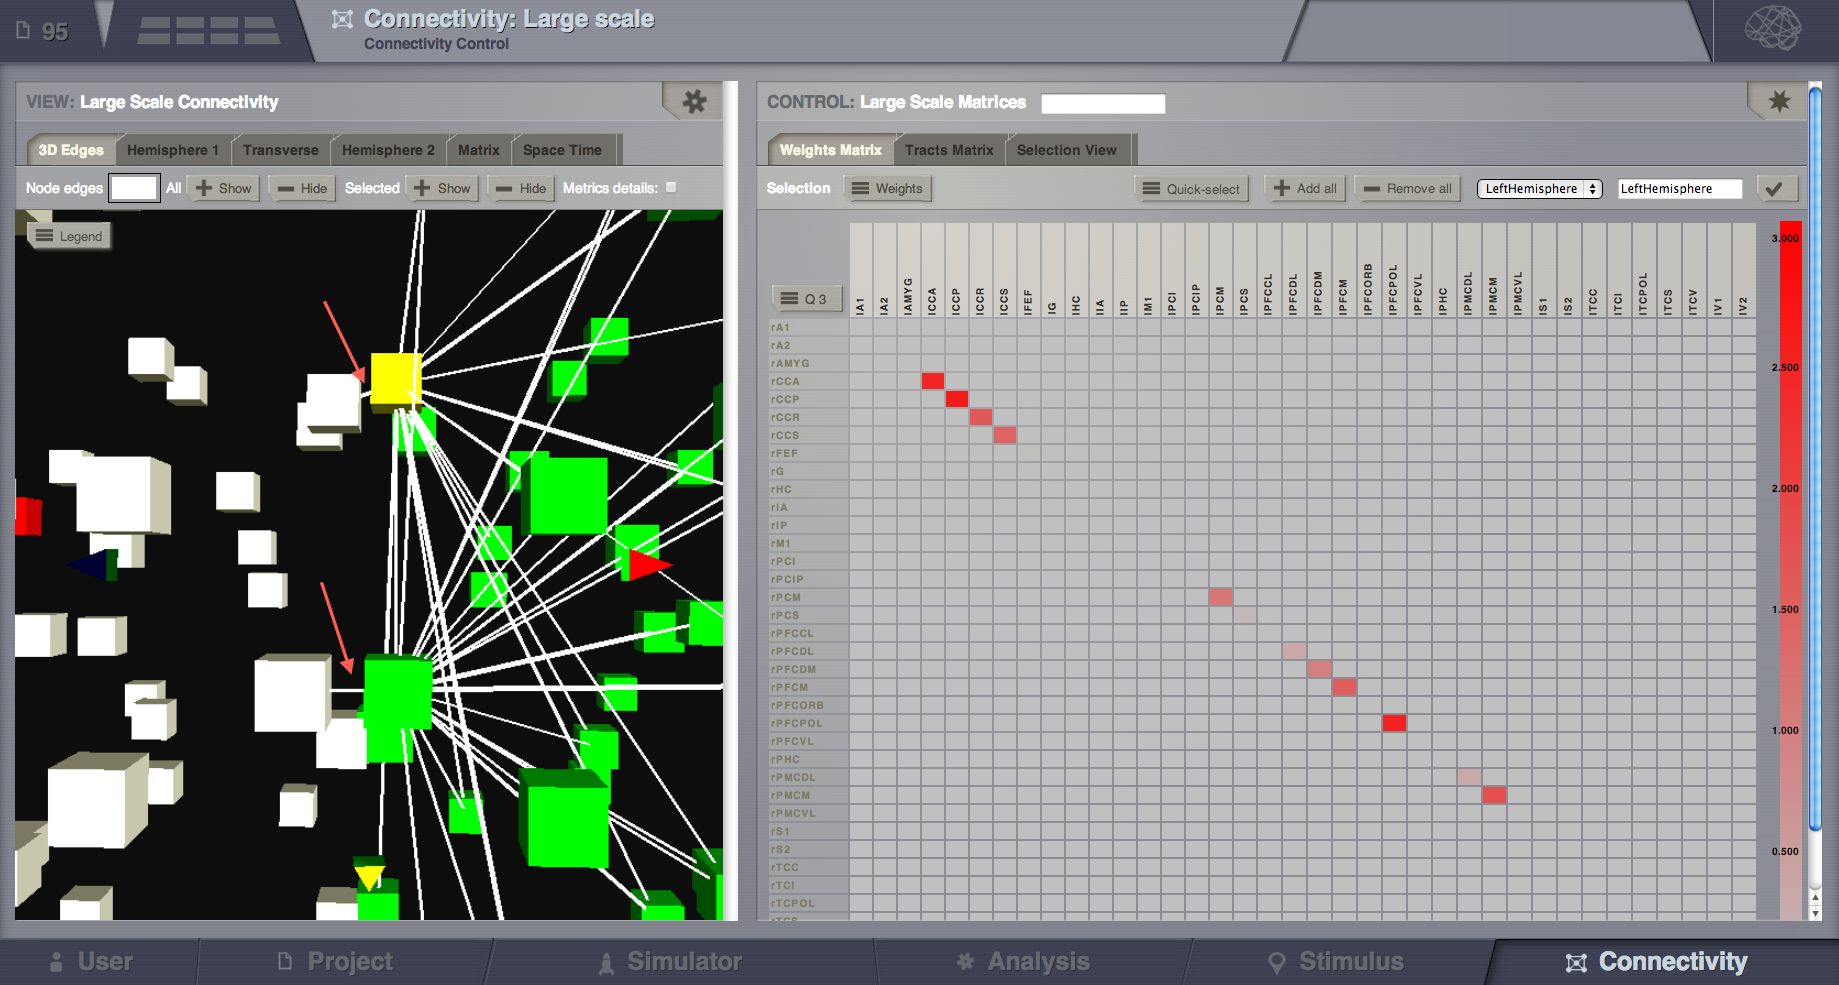
\includegraphics[width=\linewidth]{steps_Connectivity_ShowConnections.png}%
  \caption{Long-range connectivity editor}%
  \label{fig:fig}%
\end{figure}


\section{Results}\label{sec:results}

If the time-series were processed in matlab or python to obtain certain
figures like Fig.~\ref{fig:fig_results}, then they should be reproducible.
Provide a code snippet to reproduce the figure. Add some conclusions.

\begin{figure}[h]
  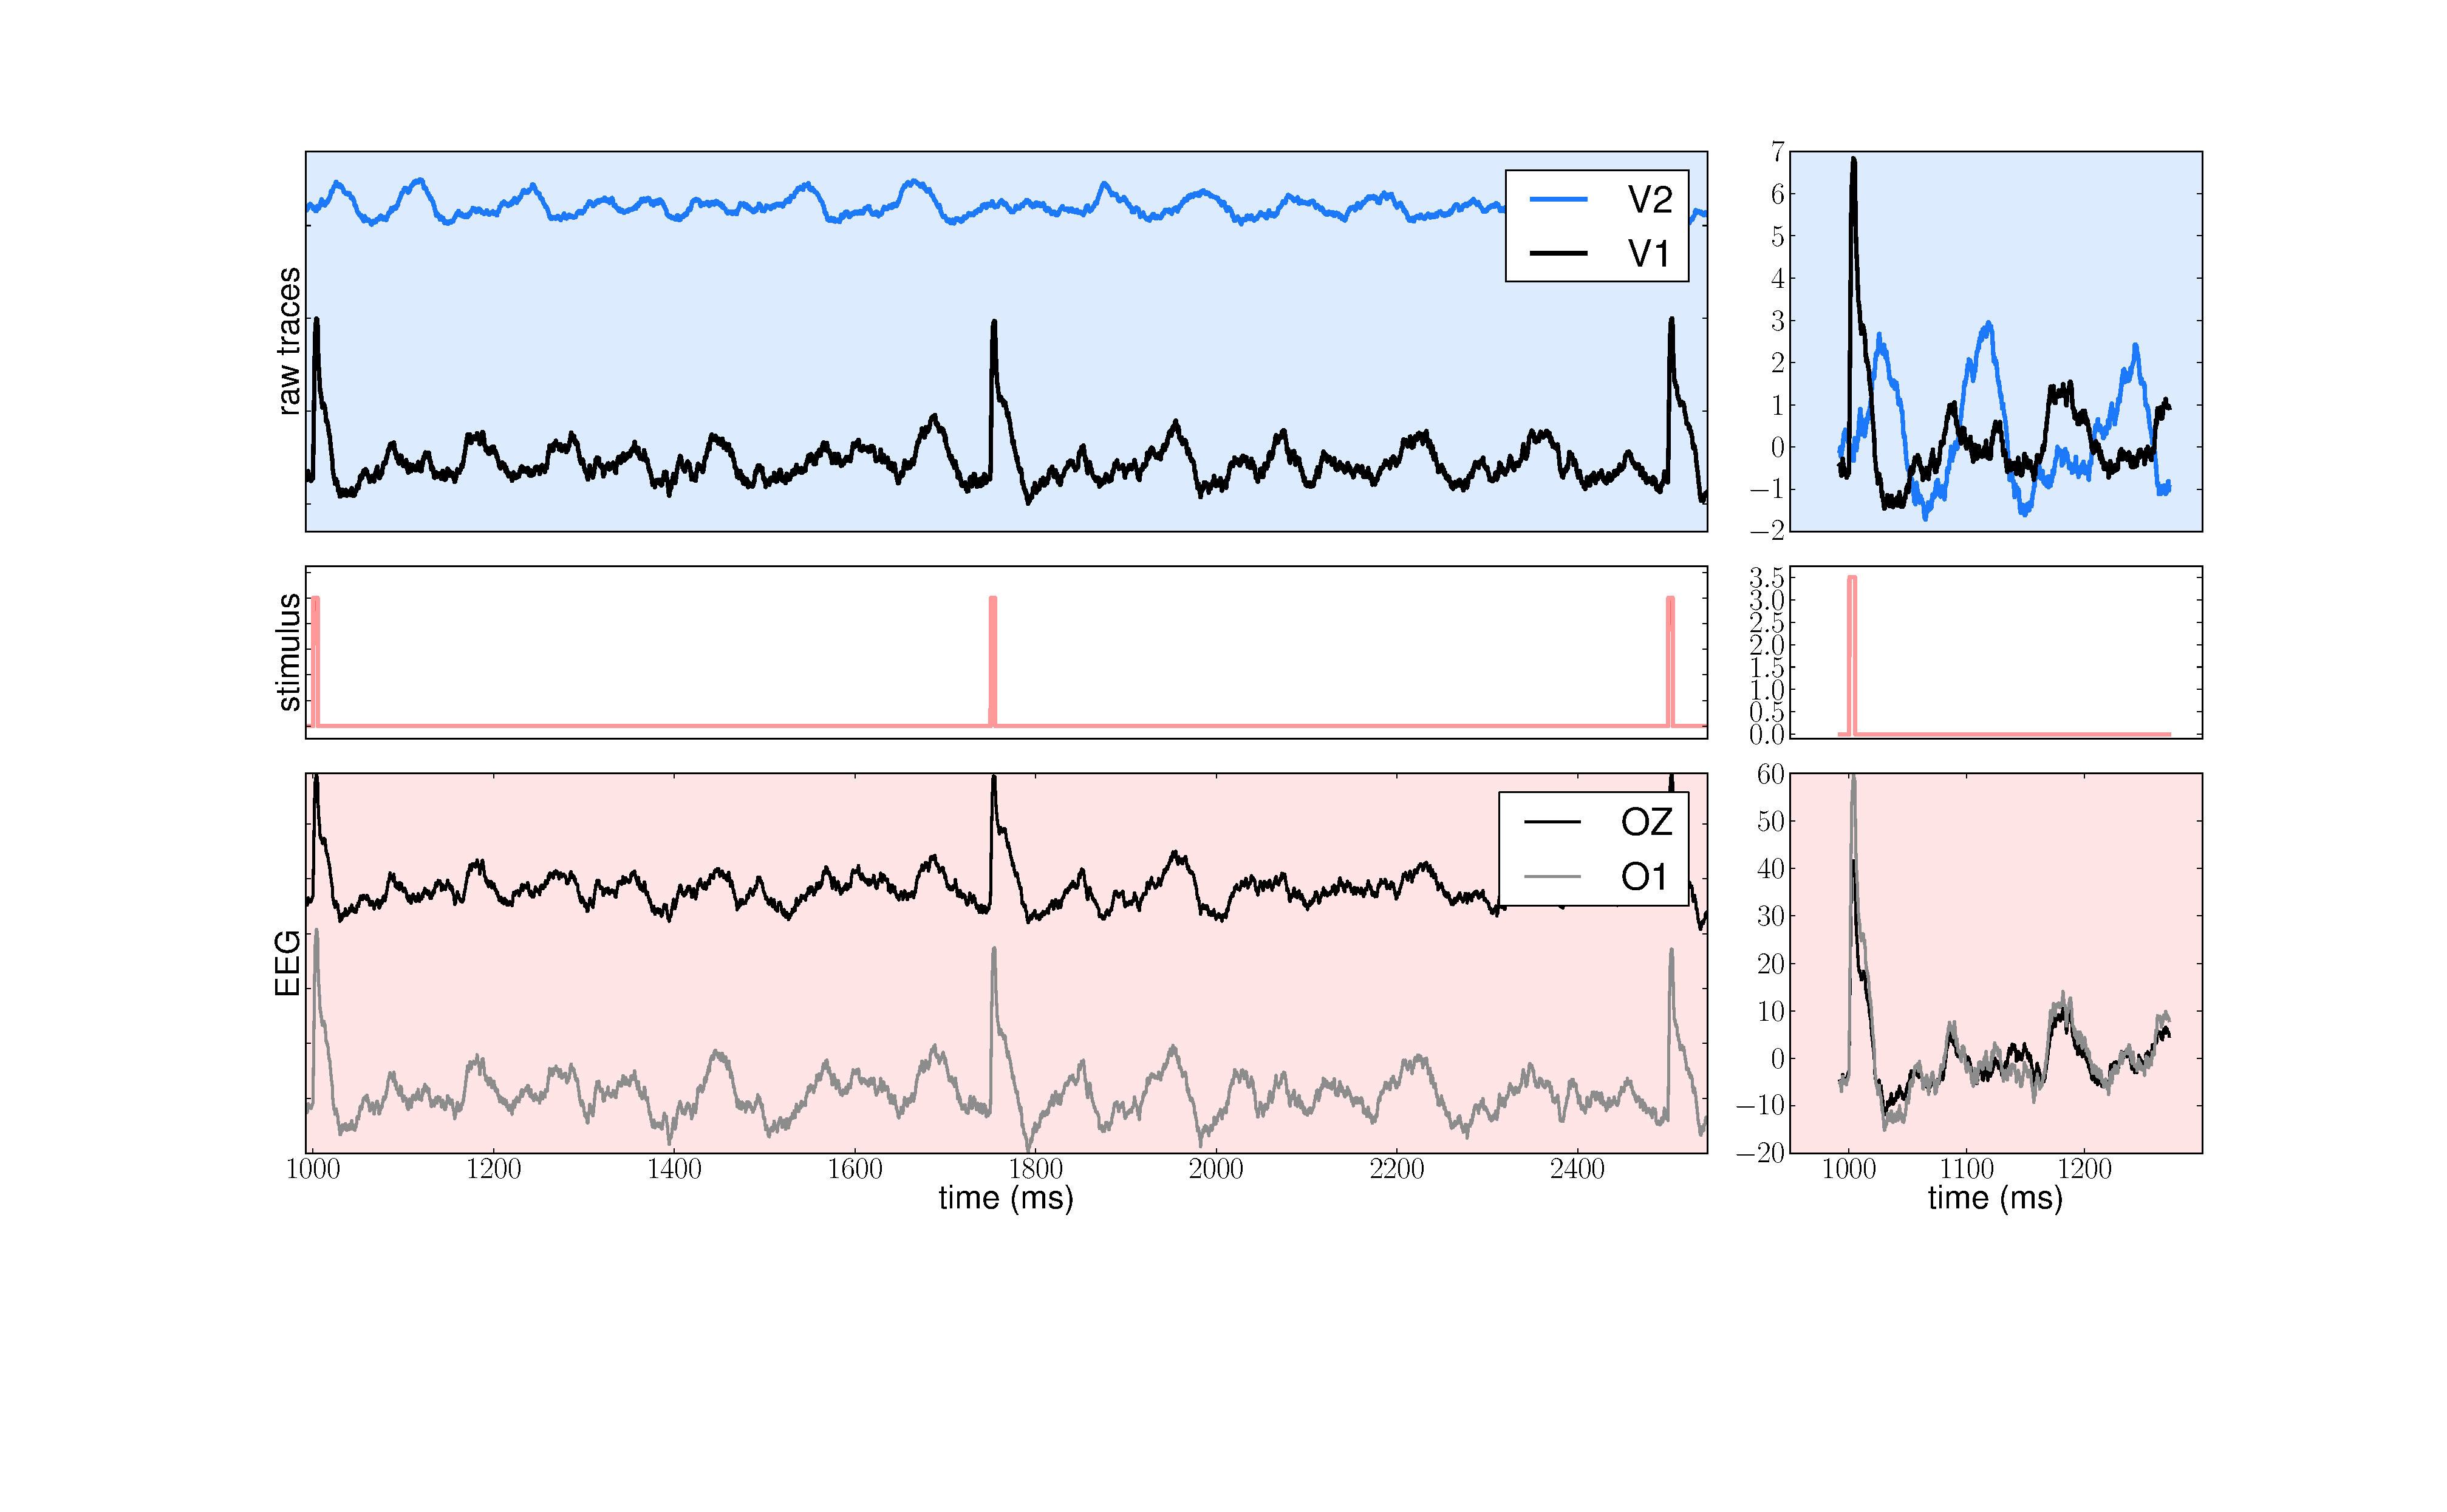
\includegraphics[width=\linewidth]{results_Example_ER_stochastic.pdf}%
  \caption{Evoked Responses}%
  \label{fig:fig_results}%
\end{figure}


\section{More Documentation}\label{sec:more-doc}
For more documentation on The Virtual Brain, please see the following articles \cite{Sanz-Leon_2013, Spiegler_2013, Jirsa_2010b}


\section{Support}\label{sec:support}

The official TVB webiste is \url{www.thevirtualbrain.org}.  
All the documentation and tutorials are hosted on \url{the-virtual-brain.github.io}.
You'll find our public \smallcaps{git} repository at \url{https://github.com/the-virtual-brain}. For questions and bug reports we have a users group \url{https://groups.google.com/forum/#!forum/tvb-users}

\bibliography{tvb_references}
\bibliographystyle{plainnat}

\end{document}